\documentclass[notoc, tikz]{tufte-handout}

\usepackage{amssymb,amsmath,amsthm}
\usepackage{bbm}
\usepackage{xifthen}
\usepackage{natbib}
\usepackage{xcolor}
\usepackage{colortbl}
\usepackage{mdframed}
\usepackage{graphicx} 
\usepackage{accents}
\usepackage{booktabs}
\usepackage{nicefrac}
\usepackage{tabu} %
\usepackage{caption}
\usepackage{cite}
\usepackage{enumitem}
\usepackage{cancel}
\usepackage{tcolorbox}
\usepackage{soul} %

\usepackage{etoolbox}
\appto\appendix{\addtocontents{toc}{\protect\setcounter{tocdepth}{1}}}
\appto\listoffigures{\addtocontents{lof}{\protect\setcounter{tocdepth}{1}}}
\appto\listoftables{\addtocontents{lot}{\protect\setcounter{tocdepth}{1}}}


\usepackage[ruled,linesnumbered]{algorithm2e}
\SetAlgorithmName{Pseudocode}{pscode}{List of Pseudocodes}

\newcommand{\dt}{{\Delta{t}}}

\setcounter{secnumdepth}{3} %

\setlength{\emergencystretch}{3em}  %
\providecommand{\tightlist}{%
  \setlength{\itemsep}{0pt}\setlength{\parskip}{0pt}}

\def\subsubsection{\subsection}

\DeclareRobustCommand{\[}{\begin{equation}}
\DeclareRobustCommand{\]}{\end{equation}}

\let\Tuftemarginnote\marginnote
\let\marginnote\relax
\usepackage{marginnote}
\let\MarginNote\marginnote
\let\marginnote\Tuftemarginnote



\def\mathnote#1{%
  \tag*{\rlap{\hspace\marginparsep{\parbox[t]{\marginparwidth}{\footnotesize#1}}}}%
}
\def\mathnotes#1{%
  \tag*{\rlap{\hspace\marginparsep\smash{\parbox[t]{\marginparwidth}{\footnotesize#1}}}}%
}
\def\mathnoteps#1{%
  \tag*{\rlap{\hspace\marginparsep{\parbox[t]{\marginparwidth}{\footnotesize#1}}}}%
}


\usepackage[hyperpageref]{backref}
\definecolor{mydarkblue}{rgb}{0,0.08,0.45}
\hypersetup{ %
    colorlinks=true,
    linkcolor=mydarkblue,
    citecolor=mydarkblue,
    filecolor=mydarkblue,
    urlcolor=mydarkblue,
    pdfview=FitH,
}

\renewcommand\backrefxxx[3]{%
  \hyperlink{page.#1}{$\uparrow$#1}%
}


\newcommand{\half}{\nicefrac{1}{2}}
\newcommand{\1}{\mathbbm{1}}
\DeclareMathOperator*{\argmin}{argmin}
\DeclareMathOperator*{\argmax}{argmax}
\newcommand{\x}{\times}
\newcommand{\Z}{\mathbb{Z}}
\newcommand{\Q}{\mathbb{Q}}
\newcommand{\R}{\mathbb{R}}
\newcommand{\N}{\mathbb{N}}
\newcommand{\F}{\mathbb{F}}
\newcommand{\E}{\mathop{\mathbb{E}}}
\renewcommand{\bar}{\overline}
\renewcommand{\epsilon}{\varepsilon}
\newcommand{\eps}{\varepsilon}
\newcommand{\nullset}{\emptyset}
\newcommand{\set}[1]{\{#1\}}

\newcommand{\flowto}[1]{\overset{#1}{\hookrightarrow} }
\newcommand{\goto}[1]{\overset{#1}{\longrightarrow} }
\newcommand{\vtxo}{v_t^{[x_0]}}
\newcommand{\vxo}{v^{[x_0]}}
\newcommand{\Tab}[2]{v^{[#1,#2]}}
\newcommand{\rflow}{\mathrm{RunFlow}}

\newcommand{\cA}{\mathcal{A}}
\newcommand{\cD}{\mathcal{D}}
\newcommand{\cZ}{\mathcal{Z}}
\newcommand{\cX}{\mathcal{X}}
\newcommand{\cY}{\mathcal{Y}}
\newcommand{\cF}{\mathcal{F}}
\newcommand{\cO}{\mathcal{O}}
\newcommand{\cN}{\mathcal{N}}
\newcommand{\cH}{\mathcal{H}}
\renewcommand{\hat}{\widehat}
\newcommand{\wt}{\widetilde}

\newtheorem{lemma}{Lemma}
\newtheorem{remark}{Remark}
\newtheorem{theorem}{Theorem}
\newtheorem{claim}{Claim}
\newtheorem{definition}{Definition}
\newtheorem{corollary}{Corollary}
\newtheorem{problem}{Problem}
\newtheorem{fact}{Fact}

\usepackage{silence}
\WarningFilter*{latex}{Marginpar on page \thepage\space moved}
\WarningFilter*{caption}{The option `hypcap=true' will be ignored}
%\geometry{showframe}% for debugging purposes -- displays the margins
\usepackage{hyperref}
\usepackage{pdfpages}
\setkeys{Gin}{width=\linewidth,totalheight=\textheight,keepaspectratio}

\title{Retrieval Augmented Generation}
\author[]{Pol Pastells}
\date{\today}  % if the \date{} command is left out, the current date will be used

\usepackage{units}
\usepackage{multicol}
\usepackage{todonotes}

\newcommand{\doccmd}[1]{\texttt{\textbackslash#1}}% command name -- adds backslash automatically
\newcommand{\docopt}[1]{\ensuremath{\langle}\textrm{\textit{#1}}\ensuremath{\rangle}}% optional command argument
\newcommand{\docarg}[1]{\textrm{\textit{#1}}}% (required) command argument
\newenvironment{docspec}{\begin{quote}\noindent}{\end{quote}}% command specification environment
\newcommand{\docenv}[1]{\textsf{#1}}% environment name
\newcommand{\docpkg}[1]{\texttt{#1}}% package name
\newcommand{\doccls}[1]{\texttt{#1}}% document class name
\newcommand{\docclsopt}[1]{\texttt{#1}}% document class option name


\newcommand{\fakesection}[1]{%
  \par\refstepcounter{section}% Increase section counter
  \addcontentsline{toc}{section}{\protect\numberline{\thesection}#1}% Add section to ToC
  % Add more content here, if needed.
}

\begin{document}

\maketitle

\begin{abstract}
\noindent This paper presents an introduction to Retrieval Augmented Generation (RAG), a technology that enhances Large Language Models by combining them with information retrieval systems. We analyze the three fundamental components of RAG systems: indexing, retrieval, and generation. We investigate multi-modal retrieval capabilities, exemplified by ColPali, through practical implementation examples. Finally, we discuss RAG's position in the evolving landscape of information retrieval, particularly in relation to emerging long-context language models.
\end{abstract}



\tableofcontents
%\printclassoptions

% ==============================================================

\section{Introduction}

Large Language Models (LLMs) have demonstrated remarkable capabilities in generating human-like text and reasoning about diverse topics. However, they face significant limitations: their knowledge is static (frozen at training time), they can hallucinate or generate incorrect information, and they lack transparency in their responses. Furthermore, they cannot access private or organization-specific information unless it was part of their training data.

Retrieval Augmented Generation (RAG) emerged as a powerful solution to these challenges. RAG combines the generative capabilities of LLMs with dynamic information retrieval systems, allowing models to ground their responses in specific documents or knowledge bases. This approach offers several key advantages:

\begin{itemize}
    \item \textbf{Up-to-date information:} RAG can access and utilize the latest documents and data, unlike static LLM knowledge.
    \item \textbf{Verifiable responses:} By citing specific sources, RAG enables fact-checking and transparency.
    \item \textbf{Domain adaptation:} Organizations can leverage their private documents and knowledge bases.
    \marginnote{A more correct term for hallucination from the medical point of view may be \textbf{confabulation} \citep{smith2023hallucination}.}
    \item \textbf{Reduced hallucination:} Grounding responses in retrieved documents helps prevent fabricated information.
\end{itemize}

A crucial component in RAG systems is the retrieval mechanism. While early approaches relied on traditional keyword-based search, modern systems utilize dense neural retrievers like ColBERT, that stands out for its balance between computational efficiency and retrieval quality. Colpali, building upon colBERT's architecture, provides a practical implementation that we will explore in detail through examples.

Although many types of RAG exists \citep{gao2023retrieval}, we will focus on the fundamental components. The basic RAG pipeline consists of three main stages: indexing, retrieval, and generation, each presenting its own challenges and optimization opportunities.


% ==============================================================

\section{Indexing}

The indexing phase is fundamental to RAG systems, involving the transformation of documents into searchable representations. While seemingly straightforward, this stage involves several critical decisions and techniques that significantly impact system performance.

\subsection{Document Chunking}
Documents must be divided into meaningful segments that balance information completeness with retrieval precision. Traditional approaches often relied on simple heuristics like fixed-length chunks or paragraph breaks. However, modern systems employ more sophisticated methods, such as using language models to identify semantically coherent sections. These systems often incorporate overlapping chunks to maintain context continuity and may adapt chunk sizes based on the inherent structure of the content.
\marginnote{Before chunking, an input query rewriter may be used to transform the initial query to its key information. For example, it would remove greetings and punctuation.`}

\subsection{Embedding Strategies}

The choice of embedding strategy affects both retrieval quality and system efficiency. Traditional dense embeddings compress document information into single vectors. While powerful and computationally efficient, the compression of hundreds of tokens into a single vector leads to information loss. This limitation becomes particularly apparent when trying to capture fine-grained details or generalization capabilities.

\marginnote{The Massive Text Embedding Benchmark (MTEB) maintains a comprehensive leaderboard on HuggingFace (\url{https://huggingface.co/spaces/mteb/leaderboard}), evaluating embedding models across 58 datasets, 8 tasks, and 112 languages. Current results suggest no single model achieves state-of-the-art performance across all tasks.}
Recent advances like Contextual Document Embeddings \citep{morris2024contextual} (CDE) challenge the traditional paradigm of encoding documents in isolation. Similar to how contextual word embeddings revolutionized NLP by considering surrounding words, CDE incorporates information from neighboring documents during embedding creation. This approach leads to richer representations that better capture document relationships and achieve superior performance, especially in out-of-domain scenarios, without requiring complex training techniques or large batch sizes.

ColBERT \citep{colbert} (Contextual Late Interaction BERT) represents another significant advancement in embedding strategy. Instead of compressing entire documents into single vectors, ColBERT maintains token-level representations. To manage the computational overhead, it employs a downcasting layer that projects each token into a low-dimensional space (typically 64 or 128 dimensions). Despite storing more vectors, ColBERT remains practical through aggressive quantization techniques, compressing vectors to just 2 bits while maintaining over 99\% of performance. Some implementations further reduce storage requirements through small-scale pooling, achieving 50-75\% storage reduction with minimal performance impact.

\section{Retrieval}

The retrieval phase involves finding the most relevant documents for a given query. Modern RAG systems often employ multiple retrieval methods in concert, leveraging the strengths of both classical and neural approaches.

\subsection{Classical Methods}

\marginnote{
    \textbf{TF-IDF:} Term Frequency-Inverse Document Frequency is a statistical measure evaluating word importance within a document relative to a corpus. It combines term frequency with inverse document frequency, which down-weights terms frequent across many documents. Despite its simplicity, it remains effective for keyword-based ranking.
}
BM25 (Best Match 25) remains a surprisingly robust baseline in information retrieval. 
It is an improvement over TF-IDF.
It refines the ranking process by incorporating term saturation (i.e., diminishing returns when a word appears too frequently) and document length normalization, making it more robust for information retrieval tasks than TF-IDF.
\marginnote{
    \textbf{PageRank:} Another classical retrieval approach that complements content-based methods like BM25. While BM25 focuses on term matching, PageRank analyzes document relationships, ranking items based on their connection patterns. Originally developed for web search, its principles are now used in many retrieval systems to incorporate document authority and relevance signals beyond pure content matching.
}
Despite its simplicity, BM25 offers several advantages:
it handles variable-length texts naturally, requires minimal computational resources, and avoids catastrophic failures through simple statistical analysis. The algorithm particularly shines with keyword-heavy queries and when exact matching is crucial.


SPLADE \citep{splade} (Sparse Lexical and Expansion)\footnote{There's currently a SPLADE v2 and v3.} represents an evolution of traditional lexical matching, incorporating neural networks while maintaining the benefits of sparse representations. It learns sophisticated term weighting and expansion mechanisms, effectively inferring relevant vocabulary not present in the original query. 
It is often used in hybrid retrieval systems.

\subsection{Neural Retrievers}

Traditional dense retrievers compress documents into single vectors, enabling efficient similarity search through techniques like approximate nearest neighbors. While this approach has proven effective, particularly when fine-tuned for specific domains, it inherits the limitations of aggressive information compression.

ColBERT's late interaction approach (see Figure~\ref{fig:colbert}) represents a more sophisticated retrieval mechanism. Instead of comparing single document vectors, it computes similarities between all query and document tokens using the MaxSim operator. For each query token, it identifies the most similar document token and combines these scores to determine overall relevance. This fine-grained interaction enables more nuanced matching while maintaining practical efficiency.

\begin{figure}
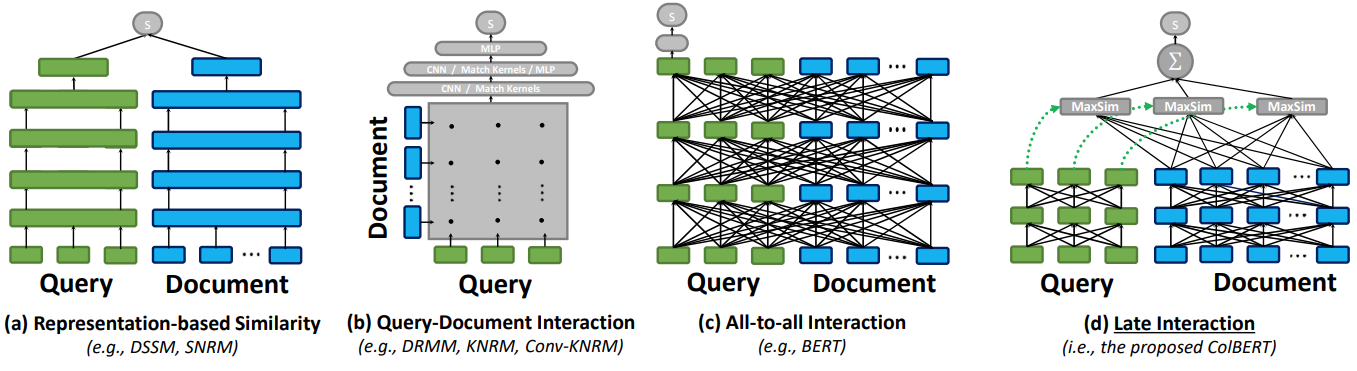
\includegraphics[width=\textwidth]{colbert.png}
\caption{Query-document matching paradigms in neural information retrieval, showing the progression from bi-encoders to late interaction models. (Taken from the ColBERT paper)}
\label{fig:colbert}
\end{figure}
\subsection{Multi-Modal Retrieval}

Recent advances, exemplified by ColPali \citep{colpali}, have extended retrieval capabilities to multi-modal content, like PDFs. By applying the late-interaction approach to image tokens generated by Vision-Language Models (VLMs), these systems can seamlessly handle text, images, and tables without extensive preprocessing. 
As illustrated in Figure~\ref{fig:colpali}, traditional document retrieval pipelines involve multiple preprocessing steps: OCR for text extraction, layout detection, chunking, and embedding generation. ColPali simplifies this process by operating directly on document images through a VLM.

\begin{figure}
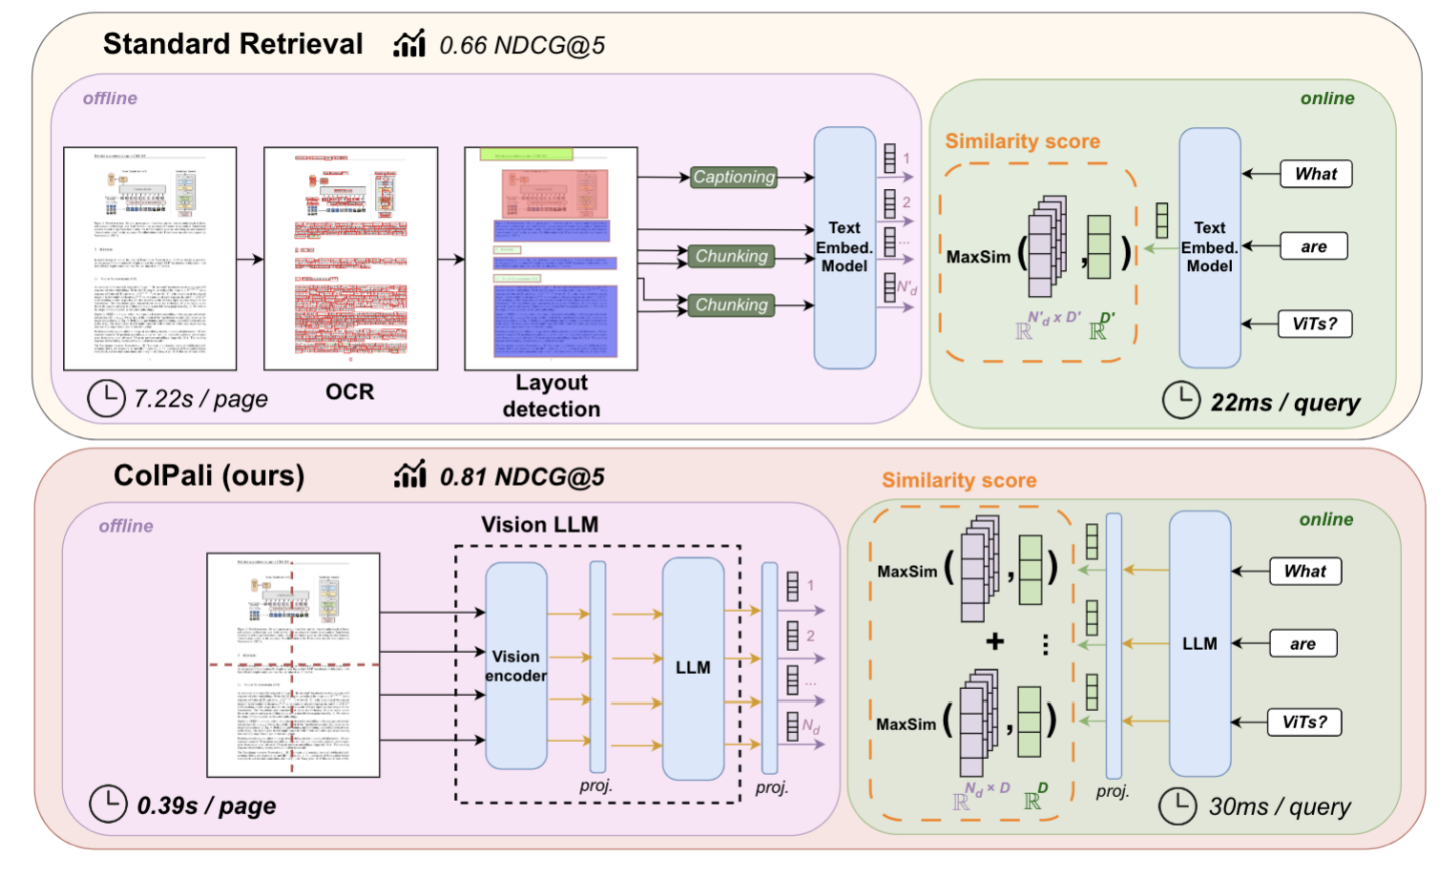
\includegraphics[width=\textwidth]{colpali.png}
\caption{Comparison between traditional PDF retrieval pipeline and ColPali's simplified approach. (Taken from the ColPali paper)}
\label{fig:colpali}
\end{figure}

\subsection{Hybrid Search}

\marginnote{
    \textbf{GraphRAG:} A specialized hybrid approach that combines knowledge graphs with LLMs. The system extracts entities, relationships, and key claims from documents to build a structured graph representation. It organizes information hierarchically, enhancing both retrieval effectiveness and result explainability.
}
Modern RAG systems typically combine multiple retrieval approaches to maximize effectiveness. 
\marginnote{
    \textbf{Reranking} consists on retrieving not just the top result, but the top \(k\) ones. After the retrieval a reranking step is run to obtain the result.
    At this step, \textbf{autocut} can be used to remove unrelated results, or to avoid comfabulations due to a low \textbf{content relevance score}, e.i., no relevant results. All of this stages can be further addapted to a specific domain.
}
A common pattern pairs lexical matching (like BM25) with semantic search methods. The lexical component ensures precise matching for keywords and explicit terms, while semantic search captures thematic relationships and implicit connections. Many systems add a final re-ranking step to refine results, particularly for applications requiring high precision.

% ==============================================================

\section{Generation}\label{generation}

The generation phase leverages an LLM to synthesize a coherent response using both the user prompt and the retrieved content. This step requires balancing between faithfully representing the retrieved information and crafting a relevant, contextual response that directly addresses the user's query.

\subsection{Prompt Engineering for Generation}

The structure of the generation prompt significantly impacts the quality of the response. Effective prompts typically frame the context for the LLM, provide explicit instructions for citation or attribution, and set clear guidelines for the response format and style. Additional parameters might include specific constraints such as word limits or required technical depth.

\subsection{Response Synthesis Strategies}

The LLM must employ several strategies to generate effective responses. First, it needs to integrate relevant details from multiple retrieved passages while maintaining coherence throughout the response. Second, the model must ensure source fidelity, accurately reflecting the retrieved information without distortion. Third, the generation process must maintain alignment with the original query, focusing on the specific aspects requested by the user. Finally, the model needs to maintain consistency when synthesizing information from multiple sources, avoiding contradictions or inconsistencies in the final response.

\subsection{Generation Challenges}

A primary concern is hallucination prevention, to ensure the model does not generate content unsupported by the retrieved context. Context length management presents another challenge, as the model must balance comprehensive information usage with its context window limitations. The generation process must also preserve relevance, maintaining focus on query-relevant information while filtering out tangential content. Additionally, the model must handle attribution accuracy, properly citing or referencing source materials in the generated response when required.

\section{Implementation examples}

An implementation of a RAG system described in this report is demonstrated in two Jupyter notebooks, included as appendices. Appendix \ref{appendix:colpali} shows how to use the ColPali model with the HuggingFace library for inference, scoring, and interpretability.
Appendix \ref{appendix:finetune} demonstrates a fine-tuning of ColPali.
Both notebooks were executed in a single RTX 4090 and are available on GitHub\footnote{\url{https://github.com/Pastells/RAG_colpali}}.



\section{Discussion and Future Developments}

The landscape of information retrieval and question answering is rapidly evolving with the emergence of long-context language models (LCLMs). While RAG systems still are the industry standard for document retrieval and question answering, recent developments in LLMs with expanded context windows, such as Mistral-NeMo (128k tokens) and Llama 3 series (131k tokens), present compelling alternatives.

Research shows that LCLMs can match or exceed RAG systems' performance in many tasks, despite not being explicitly trained for retrieval\citep{lee2024can}. However, this superior performance comes at a significant computational cost. The choice between RAG and LCLMs involves tradeoffs between accuracy, computational resources, and cost-effectiveness, as demonstrated by comparisons between the two approaches\citep{li2024retrieval}.

RAG systems maintain several advantages that suggest their continued relevance:
\begin{itemize}
    \item Cost-effectiveness for repeated queries on the same document set
    \item Ability to provide precise citations and references
    \item Better handling of focused, specific tasks without context overload
    \item Scalability to larger document collections without degradation in precision
\end{itemize}

Looking forward, hybrid approaches that combine RAG and LCLMs, such as query routing based on model self-reflection\citep{li2024retrieval}, may offer the best of both worlds. These systems can optimize for both performance and cost, while maintaining the benefits of explicit retrieval when needed.

Rather than viewing RAG as a temporary solution, it's more accurate to consider it a complementary technology that will continue to evolve alongside advances in LLMs. The future likely lies in intelligent systems that can dynamically choose between or combine these approaches based on specific use cases and requirements.


% ==============================================================

% \section{Resources} % left as easter-egg

% \citep{lewis2020retrieval}

% \begin{itemize}
% \item
%   Jurafsky 14 as background
% \item
%   RAG++ course: https://www.wandb.courses/courses/rag-in-production
% \item
%   RAG is more than dense embeddings - Ben Clavié
% \item
%   codecamp video: https://www.youtube.com/watch?v=sVcwVQRHIc8
% \item
%   Deeplearning.ai courses:

%   \begin{itemize}
%   \item
%     https://www.deeplearning.ai/short-courses/building-evaluating-advanced-rag/
%   \item
%     https://www.deeplearning.ai/short-courses/multimodal-rag-chat-with-videos/
%   \item
%     https://www.deeplearning.ai/short-courses/advanced-retrieval-for-ai/
%   \item
%     https://www.deeplearning.ai/short-courses/retrieval-optimization-from-tokenization-to-vector-quantization/
%   \end{itemize}
% \end{itemize}


\bibliography{main}
\bibliographystyle{plainnat}


\newpage
\appendix
\fakesection{Using ColPali}\label{appendix:colpali}
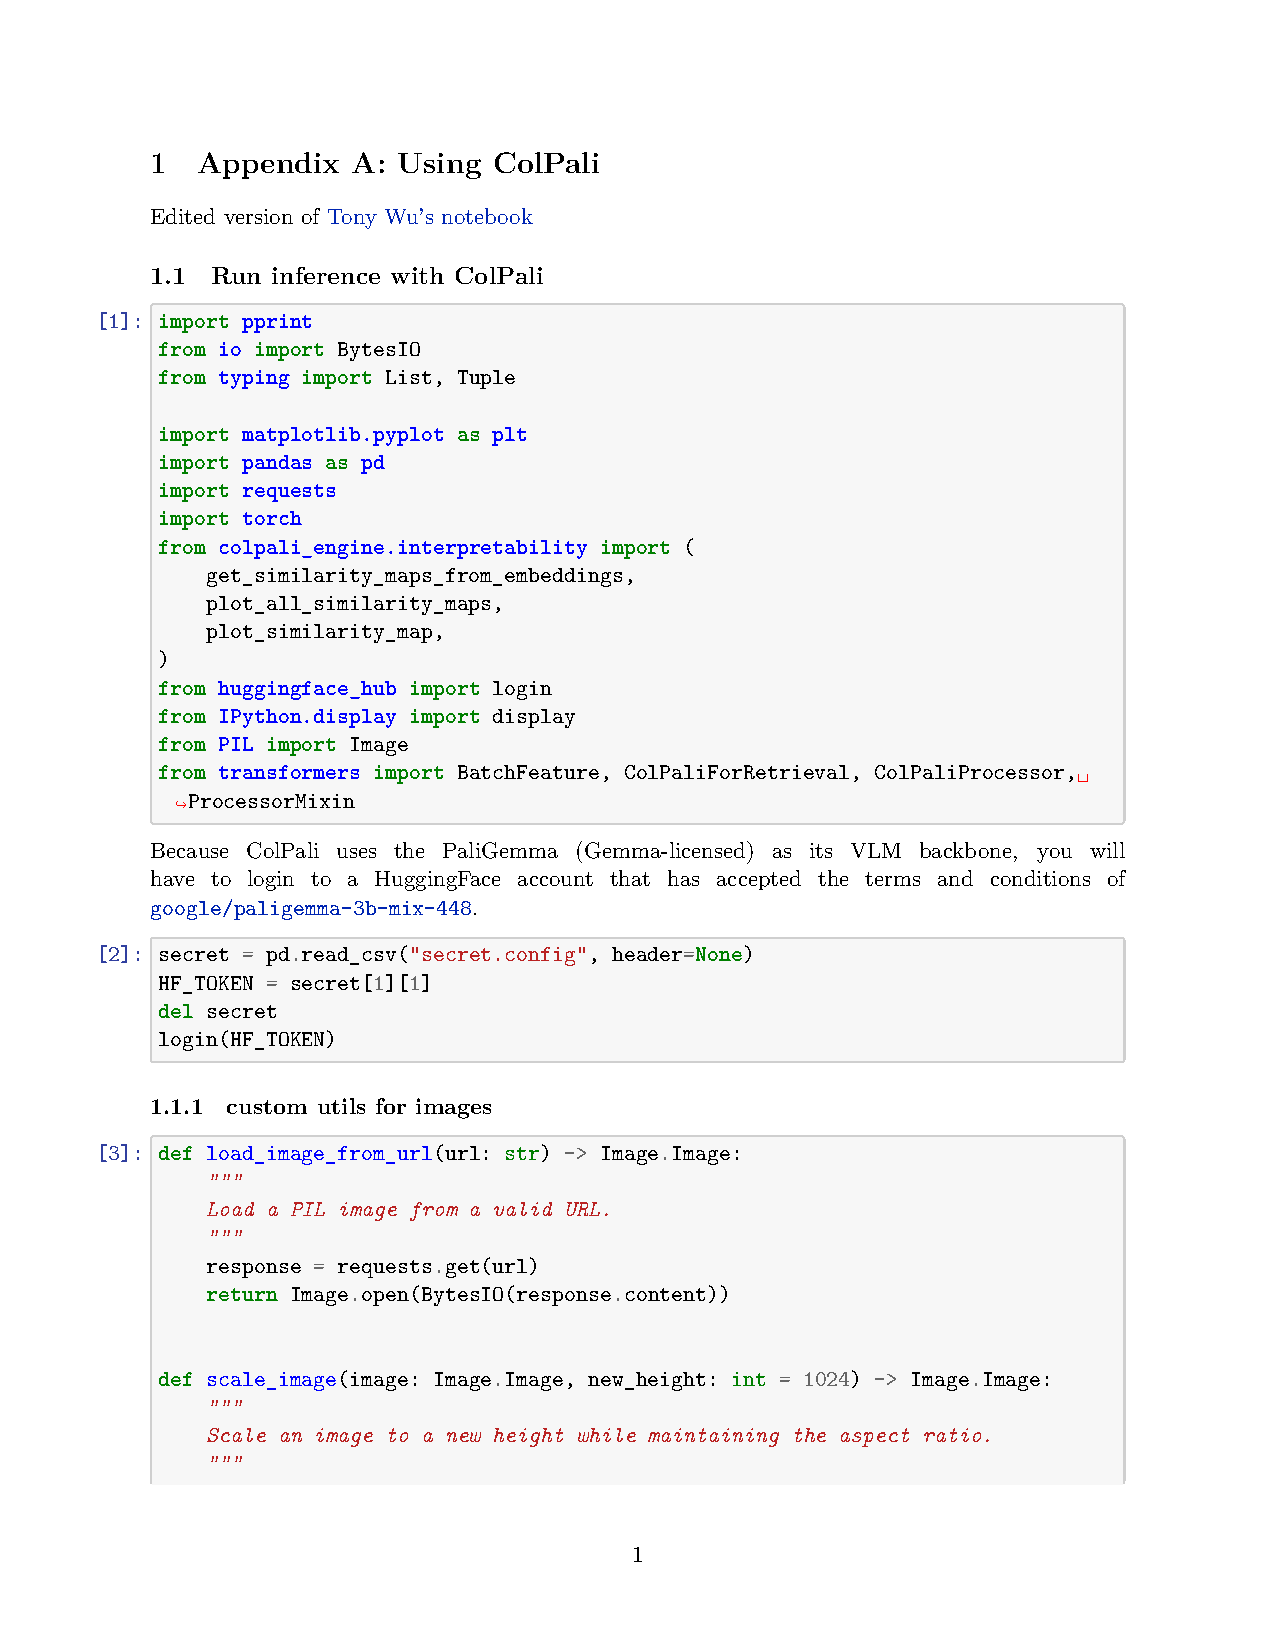
\includepdf[pages=-]{using_colpali.pdf}
\fakesection{Fine-tuning ColPali}\label{appendix:finetune}
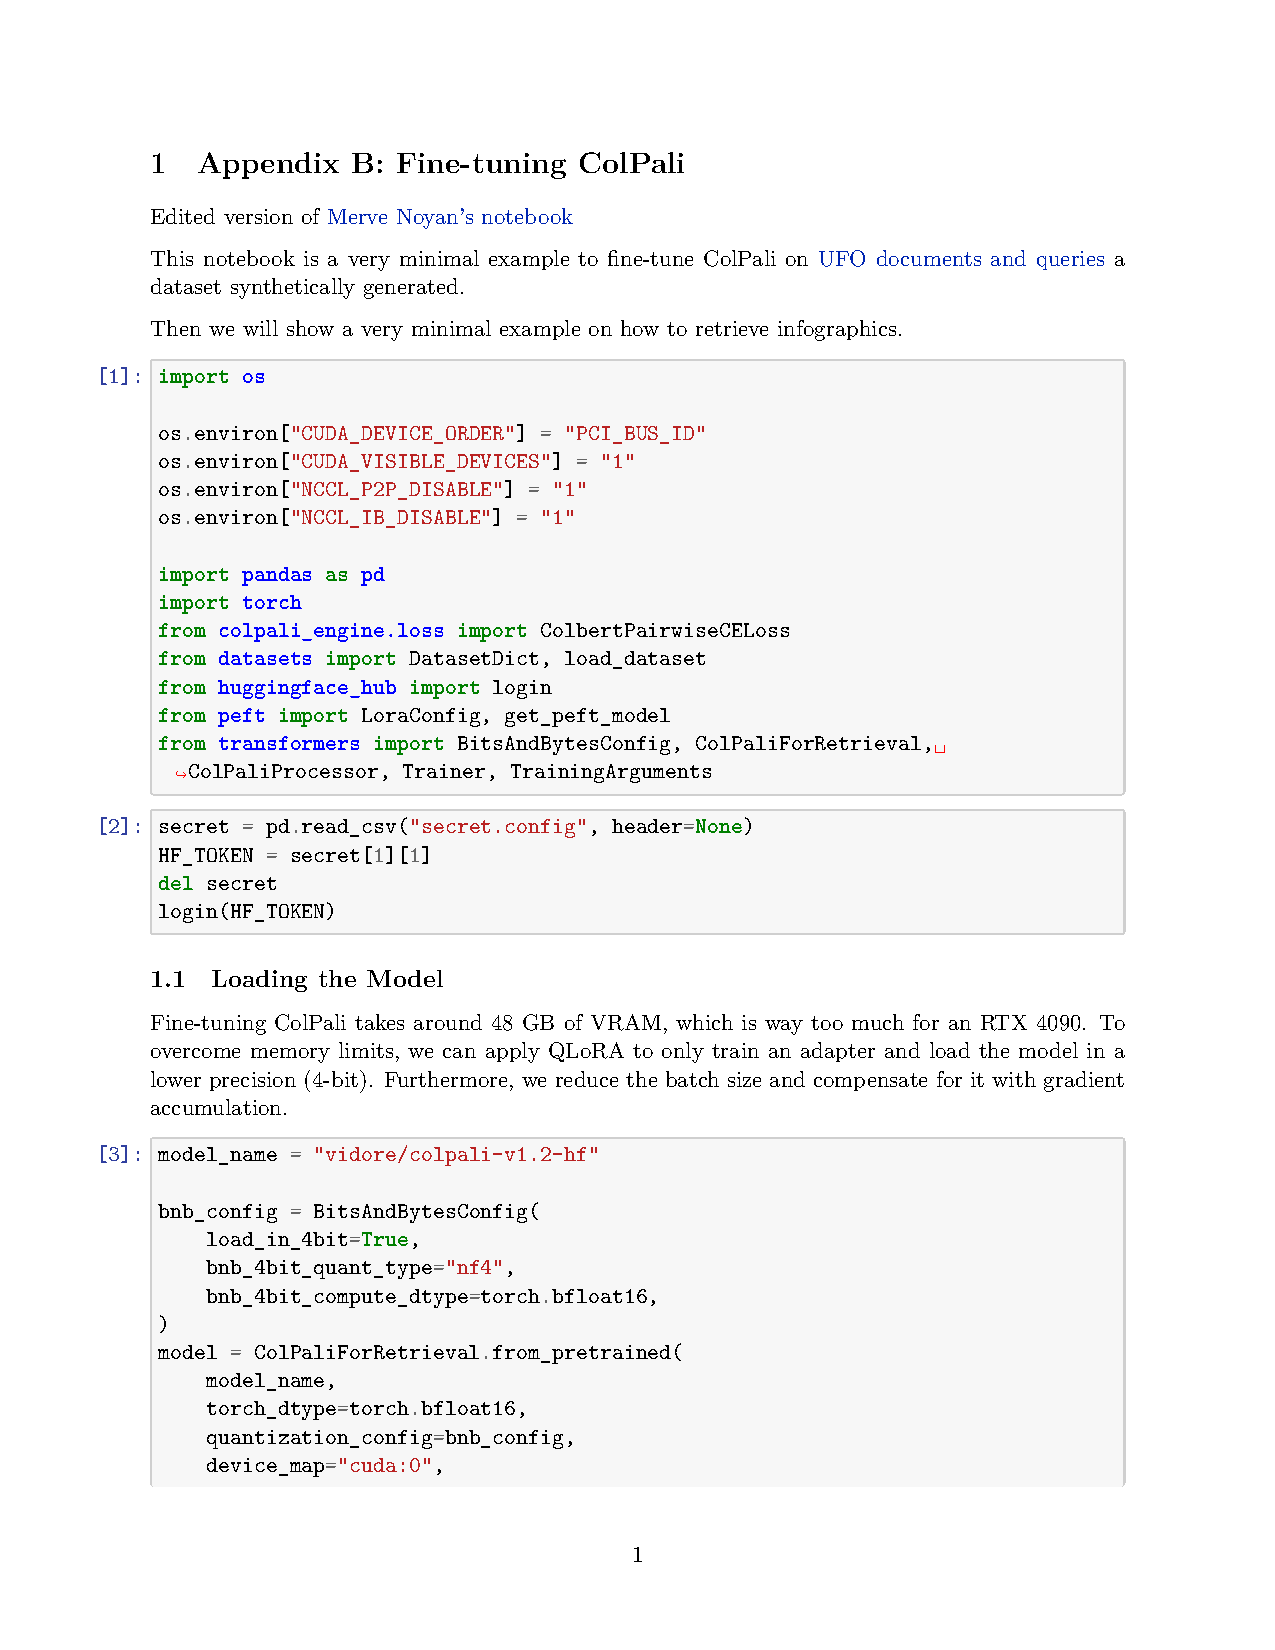
\includepdf[pages=-]{finetuning_colpali.pdf}

\end{document}